\documentclass[../main.tex]{subfiles}

\begin{document}
\subsection{}
\say{\textbf{För att det skall vara möjligt att konstruera generella algoritmer,
måste den beskrivningsmetod man använder ha förmåga att uttrycka tre konstruktioner,
även kallade kontrollstrukturer. Dessa är sekvens, selektion och iteration.
Förklara var och en av de tre kontrollstrukturerna, dvs. vad innebär sekvens, selektion resp. iteration?}}
\subsubsection{Hur uttrycker man sekvenser i Java? Skriv ett exempel (källkod).}
\begin{lstlisting}[language=java]
public class Temperature {
  public static void main(String[] args) {
  
    String input = JOptionPane.showInputDialog
    ("Enter temperature in (F): ");
    
    double f = Double.parseDouble(input);
    double c = (f - 32) * 5 / 9;
    
    JOptionPane.showMessageDialog
    (null,
    f + " degrees F " + " equals " + c + " degrees C");
  }
}
\end{lstlisting}

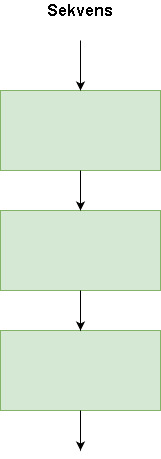
\includegraphics[width=4cm, height=5cm]{sec1/Figs/sekvens.jpg}

\newpage

\subsubsection{Hur uttrycker man selektion i Java? Skriv ett exempel (källkod).}
\begin{lstlisting}[language=java]
public class Selection {
    public static void main(String[] args) {

        String personalSerialCode = "19930609-1337";
        int sexDigit = Character.getNumericValue
        (personalSerialCode.charAt(11));

        if (sexDigit % 2 == 0)
            System.out.println("You are female");
        else
            System.out.println("You are male");
    }
}
\end{lstlisting}

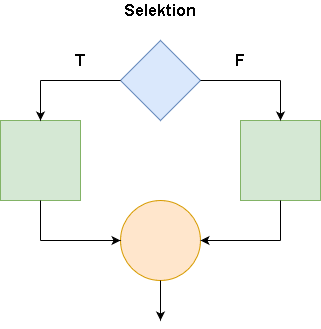
\includegraphics[width=4cm, height=5cm]{sec1/Figs/selektion.png}

\newpage

\subsubsection{Hur uttrycker man iteration i Java? Skriv ett exempel (källkod).}
\begin{lstlisting}[language=java]
public class Iteration {
    public static void main(String[] args) {
        /* Fibonacci */
        int n = 10, t1 = 0, t2 = 1;
        System.out.print("First " + n + " terms: ");

        for (int i = 1; i <= n; ++i)
        {
            System.out.print(t1 + " + ");

            int sum = t1 + t2;
            t1 = t2;
            t2 = sum;
        }
    }
}
\end{lstlisting}

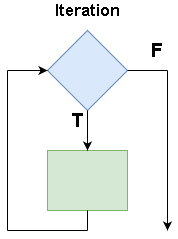
\includegraphics[width=4cm, height=5cm]{sec1/Figs/iteration.png}
\end{document}